% === Begin Label Data ===
% ID: 754
% 难度星级: 
% 标签: 
% 备注: 
% 组卷引用次数: 0
% === End  Label Data ===

\begin{problem}{2021}{G}{上海卷}{16}{不等式}
两两不同的 $x_1,x_2,x_3,y_1,y_2,y_3$ 满足 $x_1+y_1=x_2+y_2=x_3+y_3$, 且满足 $x_1<y_1,x_2<y_2$, $x_3<y_3,x_1y_1+x_3y_3=2x_2y_2>0$. 下列一定成立的是: (\hspace{1cm})
\begin{choices}
\choice{{${x_1+x_3>2x_2}$}}
\choice{{${x_1+x_3<2x_2}$}}
\choice{{${x_1x_3>x_2^2}$}}
\choice{{${x_1x_3<x_2^2}$}}
\end{choices}

已知条件中出现了大量两个变量的和与积, 进而联想到一元二次方程, 因此考虑利用抛物线数形结合来解决它:

设 $x_1+y_1=x_2+y_2=x_3+y_3=a$, $x_1y_1=b_1$, $x_2y_2=b_2$, $x_3y_3=b_3$, $2b_2=b_1+b_3$

作直线 $y=b_1$, $y=b_2$, $y=b_3$ 与 $y=-x^2+ax$ 相交, 标出题目有关交点的横坐标:
\end{problem}

\begin{answer}
A
\end{answer}

\begin{solutions}

\begin{tikzpicture}[line cap=round,line join=round,scale=0.6]
\usetikzlibrary{calc}

% --- parameters (schematic) ---
\def\a{8.0}    % parabola y = -x^2 + a x
\def\bOne{12}  % y=b1 (top line)
\def\bTwo{6}   % y=b2 (middle line)
\def\bThree{2} % y=b3 (bottom line)

% helper: intersection x of -x^2 + a x = b  -> x = (a ± sqrt(a^2-4b))/2
\pgfmathsetmacro{\dOne}{sqrt(\a*\a-4*\bOne)}
\pgfmathsetmacro{\dTwo}{sqrt(\a*\a-4*\bTwo)}
\pgfmathsetmacro{\dThree}{sqrt(\a*\a-4*\bThree)}

\pgfmathsetmacro{\xoneL}{(\a-\dOne)/2}
\pgfmathsetmacro{\xoneR}{(\a+\dOne)/2}
\pgfmathsetmacro{\xtwoL}{(\a-\dTwo)/2}
\pgfmathsetmacro{\xtwoR}{(\a+\dTwo)/2}
\pgfmathsetmacro{\xthreeL}{(\a-\dThree)/2}
\pgfmathsetmacro{\xthreeR}{(\a+\dThree)/2}

% a point on the parabola below (for the oblique segment)
\coordinate (S) at (\xthreeL,\bThree); % treat as x3 on y=b3
\coordinate (T) at (\xoneL,\bOne);     % treat as x1 on y=b1

% --- draw the three horizontal lines ---
\draw[thick] (-0.2,\bOne) -- (\a+0.6,\bOne);
\draw[thick] (-0.2,\bTwo) -- (\a+0.6,\bTwo);
\draw[thick] (-0.2,\bThree) -- (\a+0.6,\bThree);

\node[right] at (\a+0.65,\bOne) {$y=b_1$};
\node[right] at (\a+0.65,\bTwo) {$y=b_2$};
\node[right] at (\a+0.65,\bThree) {$y=b_3$};

% --- parabola y = -x^2 + a x ---
\draw[thick] plot[domain=-0.2:\a+0.2,samples=200] (\x,{-(\x)*(\x)+\a*(\x)});
\node[right] at (\a-0.2,{-(\a-0.2)*(\a-0.2)+\a*(\a-0.2)}) {$y=-x^2+ax$};

% --- mark intersection points with labels x_i, y_i ---
\coordinate (X1) at (\xoneL,\bOne);
\coordinate (Y1) at (\xoneR,\bOne);
\coordinate (X2) at (\xtwoL,\bTwo);
\coordinate (Y2) at (\xtwoR,\bTwo);
\coordinate (X3) at (\xthreeL,\bThree);
\coordinate (Y3) at (\xthreeR,\bThree);

\foreach \P/\lab/\pos in {X1/$x_1$/above,Y1/$y_1$/above,X2/$x_2$/above,Y2/$y_2$/above,X3/$x_3$/below,Y3/$y_3$/below}{
  \fill (\P) circle (1.2pt);
  \node[\pos] at (\P) {\lab};
}

% --- the oblique segment (like the picture) from x3 to x1 ---
\draw[thick] (X3) -- (X1);

% --- label (x1+x3)/2 on the middle line (schematic position) ---
\pgfmathsetmacro{\xm}{(\xoneL+\xthreeL)/2}
\coordinate (M) at (\xm,\bTwo);
\fill (M) circle (1.1pt);
\node[below] at ($(M)+(0,-0.05)$) {$\dfrac{x_1+x_3}{2}$};

\end{tikzpicture}

由图可知 $x_2<\dfrac{x_1+x_3}{2}$, 选 A. 严格的代数证明如下:

设 $x_1=m-a$, $x_2=m-b$, $x_3=m-c$, $y_1=m+a$, $y_2=m+b$, $y_3=m+c$ ($a,b,c>0$)

$m^2-a^2+m^2-c^2=2(m^2-b^2)\Rightarrow 2b^2=a^2+c^2\Rightarrow 2b^2>\dfrac{(a+c)^2}{2}\Rightarrow b>\dfrac{a+c}{2}$

即 $x_1+x_3-2x_2=2b-(a+c)>0$.

$x_1x_3-x_2^2=m^2-(a+c)m+ac-m^2+2bm-b^2=-\dfrac{(a-c)^2}{2}+m(2b-a+c)$

由于 $m$ 大小正负未知, 因此无法判断 $x_1x_3-x_2^2$ 正负, 选 A.
\end{solutions}